\documentclass{article}
\usepackage{amsmath}
\usepackage{mathbbol}
\usepackage{mathtools}
\usepackage[letterpaper,top=1in,bottom=1in,left=1in,right=1in]{geometry}
\usepackage{chngcntr}
\usepackage{amssymb}
\usepackage{graphicx}
\usepackage[verbose]{placeins}
\counterwithin*{equation}{section}
\counterwithin*{equation}{subsection}
\renewcommand{\thesubsection}{\thesection.\alph{subsection}}

\title{Written Assignment 3}
\author{Daniel Detore\\CS135-B/LF}
\date{February 17, 2024}

\begin{document}

\maketitle

\section{}
\begin{align}
     & \neg r                    & $Hypothesis$                  & \\
     & q \implies r              & $Hypothesis$                  & \\
     & \neg q                    & $Modus tollens, 1,2$          & \\
     & \neg q \implies u \land s & $Hypothesis$                  & \\
     & u \land s                 & $Modus ponens, 3,4$           & \\
     & s                         & $Simplification, 5$           & \\
     & p \lor q                  & $Hypothesis$                  & \\
     & p                         & $Disjunctive syllogism, 3, 7$ & \\
     & p \land s                 & $Conjunction, 6, 8$           & \\
     & p \land s \implies t      & $Hypothesis$                  & \\
     & t                         & $Modus ponens, 9,10$          &
\end{align}

\section{}

For simplicity's sake, I will use this key to represent the given propositions:
\begin{itemize}
    \item $p$: The dorm is locked.
    \item $q$: The phone is on top of the tall bookshelf.
    \item $r$: The dorm room is odd-numbered.
    \item $s$: The phone is under the pillow.
    \item $t$: The dorm has more than 10 floors.
    \item $u$: The phone is in the bottom drawer of the desk.
\end{itemize}

This gives us the following list of statements:

\begin{itemize}
    \item[] $p \implies \neg q$
    \item[] $r \implies q$
    \item[] $p$
    \item[] $r \lor s$
    \item[] $t \implies u$
\end{itemize}
Using this list, we can deduce the following:
\begin{align}
     & p                 & $Hypothesis$                  & \\
     & p \implies \neg q & $Hypothesis$                  & \\
     & \neg q            & $Modus ponens, 1, 2$          & \\
     & r \implies q      & $Hypothesis$                  & \\
     & \neg r            & $Modus tollens, 3, 4$         & \\
     & r \lor s          & $Hypothesis$                  & \\
     & s                 & $Disjunctive syllogism, 5, 6$ &
\end{align}
We have now confirmed that $s$ must be true. If we check the key, this means that
the phone is under the pillow.

\section{}
Let us start at the contradiction form $x = \neg x$ and derive the given
formula from it. I will use $E$ to replace $x$, and introduce new variables in
reverse alphabetical order.
\begin{align*}
     & E \lor \neg E                                                                                                           & $Original proposition$ & \\
     & \equiv (D \lor E) \land (\neg D \lor E) \land \neg E                                                                    & $Resolution$           & \\
     & \equiv (B \lor E) \land (\neg B \lor D) \land (\neg D \lor E) \land \neg E                                              & $Resolution$           & \\
     & \equiv (C \lor B) \land (\neg C \lor E) \land (\neg B \lor D) \land (\neg D \lor E) \land \neg E                        & $Resolution$           & \\
     & \equiv (A \land B) \land (\neg A \lor C) \land (\neg B \lor D) \land (\neg C \lor E) \land (\neg D \lor E) \land \neg E & $Resolution$           &
\end{align*}

\section{}
To make this argument form invalid, its premises need to be true and its
conclusion needs to be false. For simplicity's sake I will make $P(x)$ and
$Q(x)$'s domains $\{T,F\}$ and they will return the value I give them.
\begin{align*}
               & \forall x( P(x) \implies Q(x)) \\
               & \neg P(a)                      \\
    \therefore & \neg Q(a)
\end{align*}
Because $\forall x( P(x) \implies Q(x))$ places the same $x$ value into both $P(x)$ and $Q(x)$, we can simplify it to $x \implies x$. This statement is a tautology. Using the same logic, $(T \land P(a)) \implies Q(a)$ (the statement implied by argument form) will be equivalent to $a \implies a$ which is, again, a tautology. With this I have proven this argument form to be a tautology and, as such, valid.

\section{}
\subsection{}
Although the \textbf{argument} put forward is true, this is not a valid
argument \textbf{form}. \\ As an example, I will replace the predicate ``The
sum of alternating digits of $ x $ is a multiple of 11'' with ``I ate an apple
for lunch.'' Then I will replace the predicate ``$ x $ is a multiple of 11''
with ``I ate lunch today.'' Here is what this substitution yields:
\begin{align*}
               & $ If I ate an apple for lunch today, then I ate lunch today.$ & \\
               & $ I did not eat an apple for lunch today.$                    & \\
    \therefore & $ I did not eat lunch today.$                                 &
\end{align*}
This form is invalid because the premises are true:
\begin{itemize}
    \item It is true that if I ate an apple for lunch today, then I ate lunch today. I
          would have eaten the apple for lunch.
    \item I did not eat an apple for lunch today.
\end{itemize}
And the conclusion is false:
\begin{itemize}
    \item I had pancakes for lunch, therefore I \emph{did} have lunch.
\end{itemize}
This new version of the argument demonstrates that this form, which is denying the antecedent rather than the consequent, is not valid.

\subsection{}
This is another invalid argument form.\\ Here is a reinterpretation of the
argument with different predicates:
\begin{align*}
               & $ Every player on the Yankees plays baseball. $ & \\
               & $ I play baseball. $                            & \\
    \therefore & $ I am on the Yankees. $                        &
\end{align*}
This form is invalid because the premises are true:
\begin{itemize}
    \item Every player on the Yankees plays baseball (no matter how well).
    \item I do play baseball.
\end{itemize}
And the conclusion is false:
\begin{itemize}
    \item I am not on the Yankees.
\end{itemize}
This new version of the argument demonstrates that this form, which is affirming the consequent rather than the antecedent, is not valid.

\section{}
This argument is invalid. It seems to be a confused interpretation of the
Resolution rule of inference. \\ Let us define some placeholder predicate
names.
\begin{align*}
    T(x) & $: $ x $ can run 10 km in $<30$ minutes.$ & \\
    S(x) & $: $ x $ is a smoker.$                    & \\
    H(x) & $: $ x $ can run 100 m in $<11$ seconds.$ &
\end{align*}
The domain of all three predicates consists of all athletes. Here is the argument
rewritten with these placeholders:
\begin{align*}
               & \neg \exists x(T(x) \land S(x))  & \\
               & \neg \exists x(S(x) \land H(x))  & \\
    \therefore & \neg \exists x( T(x) \land H(x)) &
\end{align*}
Let us find out what happens when we fill in a specific athlete Josh. Josh is not a smoker and can run at 0.75 kilometers per minute. Here is Josh's running speed graphed: \\

\begin{figure}[hbt!]
    \centering
    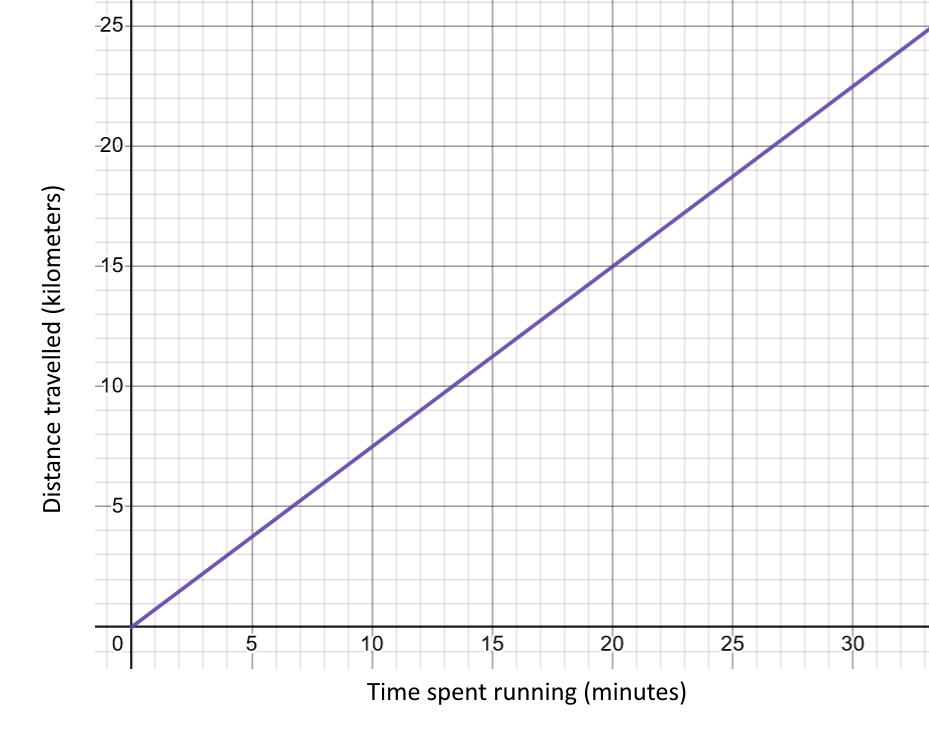
\includegraphics[width=0.7\textwidth]{justjosh}
    \caption{Distance vs.\ time graph of Josh's running speed.}
\end{figure}
\FloatBarrier

Now we can compare Josh to Tina, who runs 10 kilometers in 30 minutes, and
Hunter who runs 100 meters in 11 seconds. \\

\begin{figure}[hbt!]
    \centering
    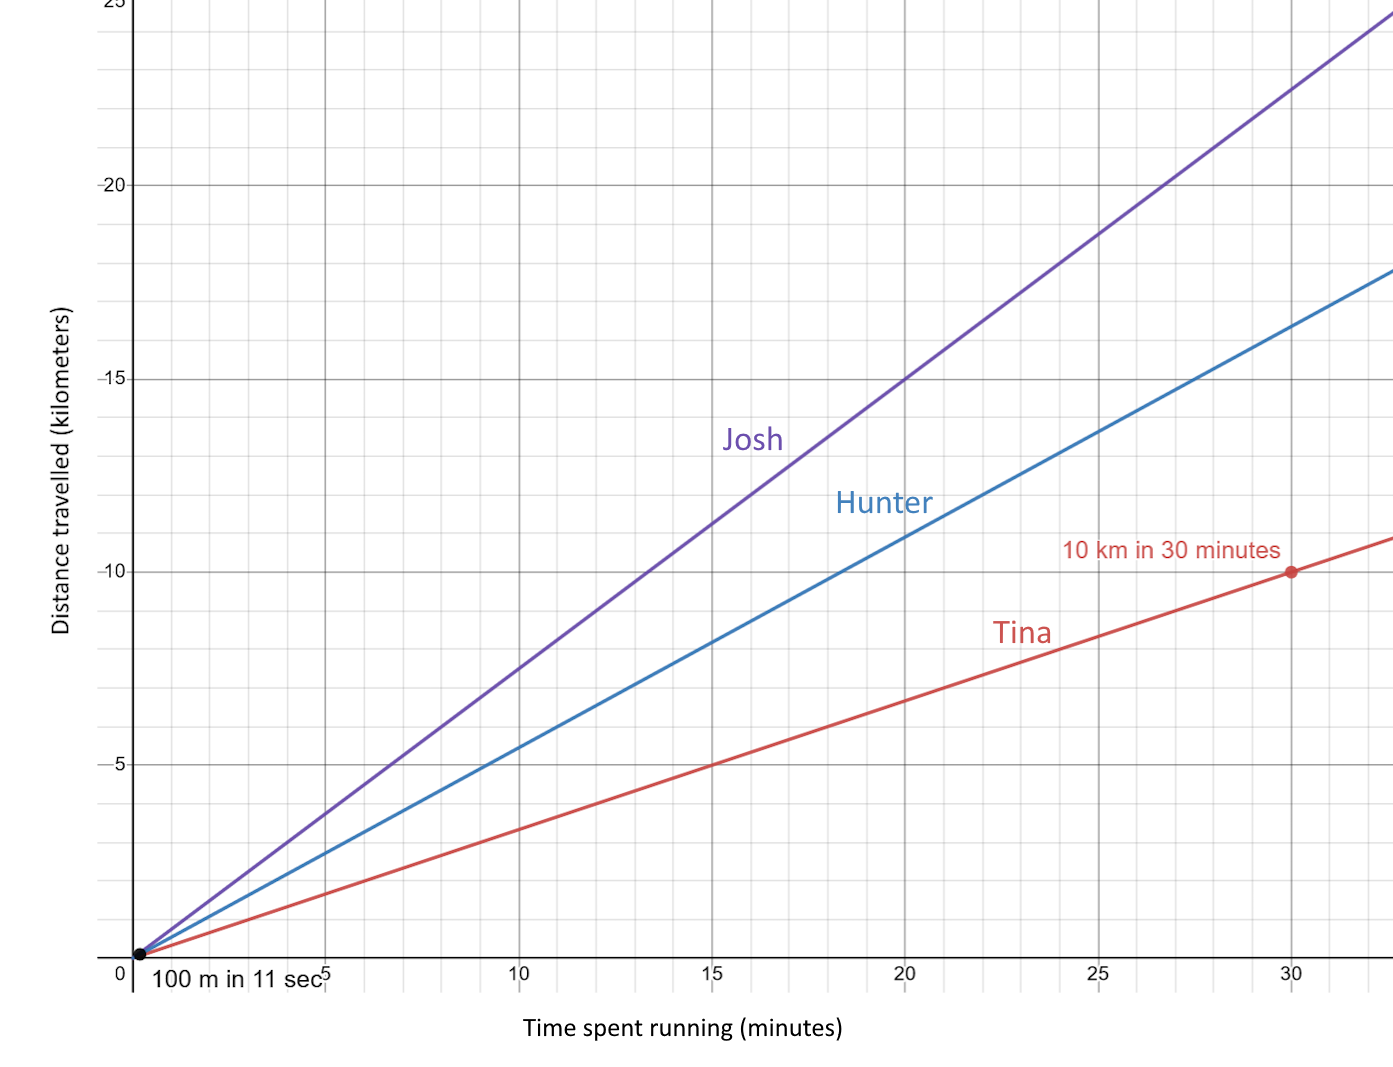
\includegraphics[width=0.7\textwidth]{allrunners}
    \caption{Distance vs.\ time graph of Tina, Hunter, and Josh's running speeds.}
\end{figure}
\FloatBarrier

We can see from this diagram that anybody, like Josh, who can run as fast or
faster than Hunter can both run 10 km in $<30$ minutes and run 100 m in $<11$
seconds, regardless of whether they smoke or not. Let us return to the argument
form I provided earlier, and place Josh into it:
\begin{align*}
               & \neg (T(Josh) \land S(Josh))  & \\
               & \neg (S(Josh) \land H(Josh))  & \\
    \therefore & \neg ( T(Josh) \land H(Josh)) &
\end{align*}
And this argument's truth values simplify as such:
\begin{align*}
               & \neg (T \land F)  & \\
               & \neg (T \land F)  & \\
    \therefore & \neg ( T \land T) &
\end{align*}
which becomes
\begin{align*}
               & T & \\
               & T & \\
    \therefore & F &
\end{align*}
which proves this argument form invalid.

\end{document}

latexmk -pvc -pvctimeoutmins=5 -pdf -pdflatex="pdflatex -interaction
nonstopmode" hw3.tex

We can use De Morgan's laws to transform the argument as such:
\begin{align*}
               & \forall x(\neg T(x) \lor \neg S(x)) \\
               & \forall x(\neg S(x) \lor \neg H(x)) \\
    \therefore & \forall x(\neg T(x) \lor \neg H(x))
\end{align*}
Let us simplify it further by looking at how these predicates can be true for one athlete:
\begin{align*}
               & \neg t \lor \neg s \\
               & \neg s \lor \neg h \\
    \therefore & \neg t \lor \neg h
\end{align*}
At this stage, it looks like the original argument form is a confusion of the Resolution rule of inference.